\subsection{Oxford}

%En este experimento decidimos realizar el traceroute hacia la universidad de Oxford, ubicada en Inglaterra. Para la realización del mismo decidimos establecer un $TTL\_MAX$ de 30 saltos, es decir que cortabamos la ejecución si no alcanzabamos el destino en, a lo sumo, 30 saltos. Por otro lado, por cada iteración de los $TTL$ emitimos una ráfaga de 30 paquetes.

En la tabla \ref{traceroute-oxford-con-ceros} podemos observar el traceroute generado. 


\begin{table}[!htbp]
\centering
\caption{Traceroute Oxford}
\label{traceroute-oxford-con-ceros}
\begin{tabular}{|c|c|c|c|}
\hline
\textbf{TTL} & \textbf{IP}       & \textbf{COUNTRY} & \textbf{OUTLIERS} \\ \hline
1            & 10.0.2.2          & Undefined        & {[}outlier{]}     \\ \hline
6            & 200.89.161.137    & Argentina        & {[}outlier{]}     \\ \hline
7            & 200.89.165.5      & Argentina        &                   \\ \hline
8            & 200.89.165.250    & Argentina        &                   \\ \hline
9            & 190.216.88.33     & Argentina        & {[}outlier{]}     \\ \hline
10           & 67.17.94.249      & Australia        & {[}outlier{]}     \\ \hline
13           & 212.187.139.166   & United Kingdom   & {[}outlier{]}     \\ \hline
14           & 146.97.33.2       & United Kingdom   & {[}outlier{]}     \\ \hline
15           & 146.97.37.194     & United Kingdom   & {[}outlier{]}     \\ \hline
16           & 193.63.108.94     & United Kingdom   &                   \\ \hline
17           & 193.63.108.98     & United Kingdom   & {[}outlier{]}     \\ \hline
18           & 193.63.109.90     & United Kingdom   &                   \\ \hline
20           & 192.76.32.66      & United Kingdom   & {[}outlier{]}     \\ \hline
21           & 129.67.242.154    & United Kingdom   & {[}outlier{]}     \\ \hline
\end{tabular}
\end{table}

Comencemos por describir la ruta generada:

Se han realizado 21 saltos hasta alcanzar el destino solicitado, de los cuales en $2/3$ de los mismos hemos obtenido respuestas del tipo $TIME\_EXCEEDED$, determinando así que el largo de nuestra ruta es de 14 saltos, y que para el tercio restante de valores del $TTL$ no hemos obtenido respuesta alguna. Como también se puede ver en la figura (pONE MAPA PUTO), y en el cuadro \ref{traceroute-oxford-con-ceros}, durante el trayecto se realizaron 3 saltos intercontinentales.

Realicemos ahora un análisis más profundo sobre los resultados obtenidos.

Lo primero que podemos notar es que la primera IP que responde corresponde a un nodo dentro de la red local, motivo por el cual no hemos podido determinar la ubicación de dicho nodo. Entendemos que el mismo se trata del gateway que separa la red LAN desde la que hemos lanzado el experimento, de internet. Esto ocurrirá en todos los experimentos, por lo que no se volverá a mencionar. 

Lo segundo que hemos notado, y que nos ha llamado poderosamente la atención, es que el método de Cimbala de detección de outliers nos ha identificado a todos los saltos con tiempo mayor a cero como outlier. Analicemos que podrían significar los ceros en este caso y veamos que podríamos hacer para afinar la búsqueda y detección de outliers.

Como mencionamos previamente, hemos decidido indicar que el tiempo de un salto es cero si, al restarle el tiempo promedio del salto anterior, el resultado es negativo. \\
Ahora bien, ¿Por qué podría ser que el tiempo de un salto diera negativo? \\
Algunos de los motivos a los que se podría deber son los siguientes:

\begin{itemize}
	\item La distancia entre los nodos es muy chica, por lo tanto, al obtener el valor promedio del salto, podemos obtener valores similares, pudiendo ser que el tiempo del salto más lejano sea menor al anterior y de esta manera obtener un salto con tiempo negativo.
	\item Las rutas para llegar de un nodo a otro no son siempre las mismas, por lo que no podemos afirmar que un salto resultante en nuestro traceroute haya sido el que se haya realizado efectivamente. Es decir, que en la ruta generada observemos que se realiza un salto del nodo A al nodo B no significa que siempre que se haya alcanzado al nodo B haya sido habiendo pasado inmediatamente antes por el nodo A. Si bien con nuestra implementación del traceroute, quedandonos en cada hop con el nodo que más veces respondió, creemos que la probabilidad de que eso si ocurra es alta, no lo podemos afirmar para todos los casos. \\
	Cabe mencionar que existe otro tipo de implementación del traceroute que resolvería este inconveniente, en donde cada nodo por el que va pasando el paquete envíado genera una respuesta para el nodo emisor, pero requiere que todos los nodos intermedios implementen dicha funcionalidad.
	\item Podría suceder también que entre los distintos $TTLs$ tengamos distintos niveles de congestión en la red, por lo que eso afectaría a los tiempos de cada hop, generando así el comportamiento descripto. \\
	Notar que en los casos anteriores también podría estar influenciando algún factor relacionado a la congestión en la red.
\end{itemize}


Mediante algunas pruebas notamos que los tiempos con valor cero nos estaban afectando a la detección de los outliers, por lo que decidimos tenerlos en cuenta para la ruta generada, pero no así para la búsqueda de los valores más extremos.

Veamos en \ref{traceroute-oxford} como resultó nuestra ruta sin contemplar los ceros recientemente mencionados.


\begin{table}[!htbp]
\centering
\caption{Traceroute Oxford}
\label{traceroute-oxford}
\begin{tabular}{|c|c|c|c|}
\hline
\textbf{TTL} & \textbf{IP}       & \textbf{COUNTRY} & \textbf{OUTLIERS} \\ \hline
1            & 10.0.2.2          & Undefined        & 			       \\ \hline
6            & 200.89.161.137    & Argentina        & {[}outlier{]}     \\ \hline
7            & 200.89.165.5      & Argentina        &                   \\ \hline
8            & 200.89.165.250    & Argentina        &                   \\ \hline
9            & 190.216.88.33     & Argentina        &                   \\ \hline
10           & 67.17.94.249      & Australia        & {[}outlier{]}     \\ \hline
13           & 212.187.139.166   & United Kingdom   & {[}outlier{]}     \\ \hline
14           & 146.97.33.2       & United Kingdom   & {[}outlier{]}     \\ \hline
15           & 146.97.37.194     & United Kingdom   &                   \\ \hline
16           & 193.63.108.94     & United Kingdom   &                   \\ \hline
17           & 193.63.108.98     & United Kingdom   &                   \\ \hline
18           & 193.63.109.90     & United Kingdom   &                   \\ \hline
20           & 192.76.32.66      & United Kingdom   & {[}outlier{]}     \\ \hline
21           & 129.67.242.154    & United Kingdom   & {[}outlier{]}     \\ \hline
\end{tabular}
\end{table}


Como podemos observar, ahora la detección de outliers nos permite realizar un mejor análisis de la situación, y por lo tanto, este razonamiento será utilizado en los próximos experimentos. Sobre 14 saltos, hemos identificado 6 saltos como outliers de los cuales solo 2 de ellos se corresponden a saltos intercontinentales, por lo tanto podríamos afirmar que los 4 restantes son falsos positivos, mientras que no se presentan casos donde se haya producido un salto entre continentes y el método no lo haya podido detectar, es decir, no tenemos casos de falsos negativos. Resumiendo, obtuvimos:

\begin{itemize}
	\item $29 \% $ de falsos positivos aprox.
	\item $0 \%$ de falsos negativos.
	\item $71 \%$ de resultados acertados aprox.
\end{itemize}

Centremonos ahora en la detección de los outliers. Para esto, observemos en la figura \ref{tiempos-oxford} los tiempos de cada salto.

\begin{figure}[!htbp]
  \centering
    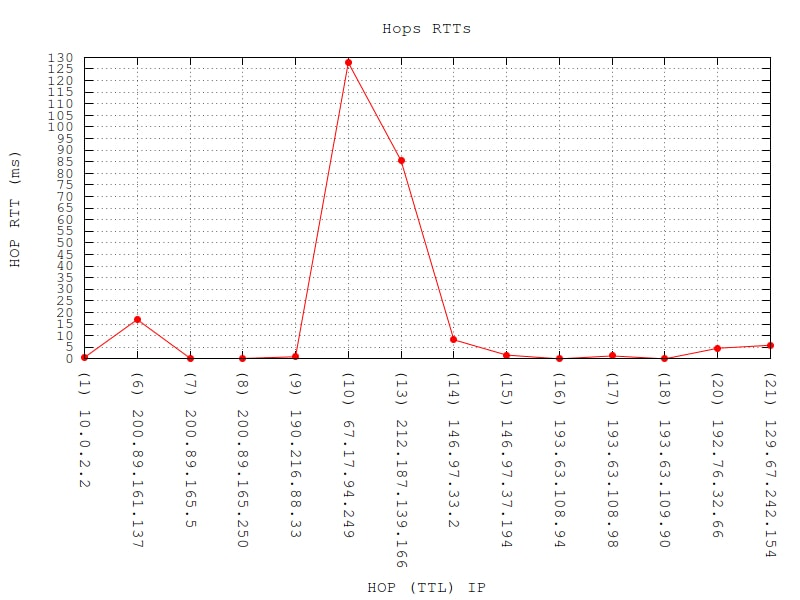
\includegraphics[scale=0.5]{imagenes/oxford-graficos/traceroute-oxford.jpg}
  \caption{Oxford- RTT hops}
  \label{tiempos-oxford}
\end{figure}


Claramente para los saltos correspondientes a los $TTLs$ 10 y 13 notamos valores muy por encima del resto. Efectivamente estos casos han sido detectados por el método de Cimbala y son justamente los únicos que se corresponden a los saltos intercontinentales.

En cuanto a los otros outliers detectados, los que se corresponden con los $TTLs$ 6, 14, 20 y 21, podemos ver como sus valores están por encima del resto, pero no de un modo tan tajante como en los casos mencionados previamente. Estos hops no solo no se corresponden a saltos entre continentes sino que han sido dentro del mismo país cada uno de ellos.


En la figura \ref{tiempos-oxford-estandarizados} decidimos reflejar los tiempos de los saltos de acuerdo a lo que propone el método de Cimbala, es decir, para cada $TTL$ tomamos $\frac{X_i - \bar{X}}{S}$, y ahora veremos la importancia de este. Por lo dicho hasta ahora, parecería que la estimaión de Cimbala es bastante poco precisa, pero observemos detenidamente esta figura. En esta, podemos apreciar que la mayoría de los puntos se sitúan un poco por encima del 0.4. Observemos entonces que Cimbala considera outlier todo  punto que se aleja de ese valor. También observemos, que si nos quedamos solo con los puntos que se encuentran por encima de este valor, obtenemos exactamente los saltos intercontinentales.


\begin{figure}[!htbp]
  \centering
    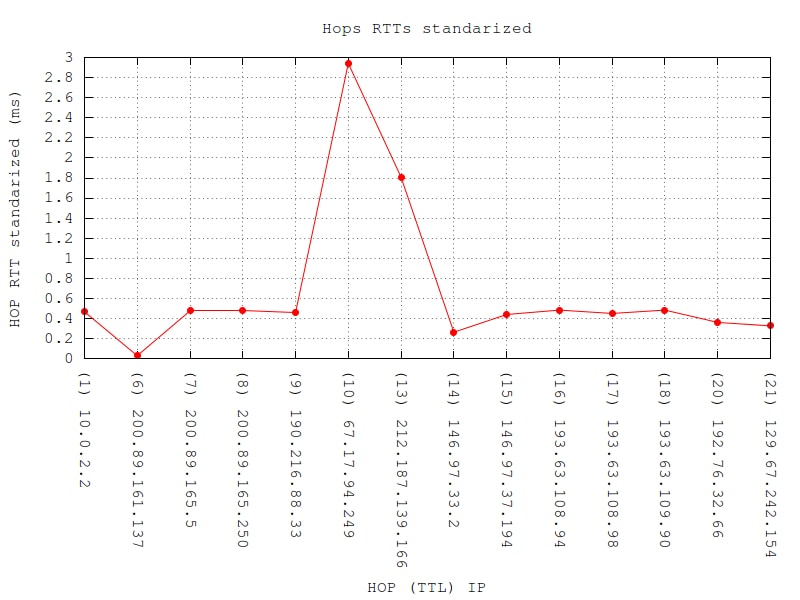
\includegraphics[scale=0.5]{imagenes/oxford-graficos/traceroute-oxford-standarized.jpg}
  \caption{Oxford- RTT hops standarized}
  \label{tiempos-oxford-estandarizados}
\end{figure}

Resumiendo, si consideramos solo los valores que en la figura \ref{fig:2} están por encima del punto de acumulaciónPONGANME UN BUEN NOMBRE, pasamos a obtener un $100\%$ de aciertos, o sea, una medición perfecta.


